\section{Vektorer og afstand}

\subsection{Fra punkt til vektor (idéen)}
Et punkt i planen kan skrives som koordinater:
\[
A = (x, y)
\]

Vi kan opfatte dette som en vektor fra origo $(0,0)$ ud til punktet:
\[
\vec{a} =
\begin{bmatrix}
x \\
y
\end{bmatrix}
\]

Altså:  
En vektor fortæller bare “hvor langt vi går i x-retning og y-retning”.

\begin{figure}[H]
    \centering
    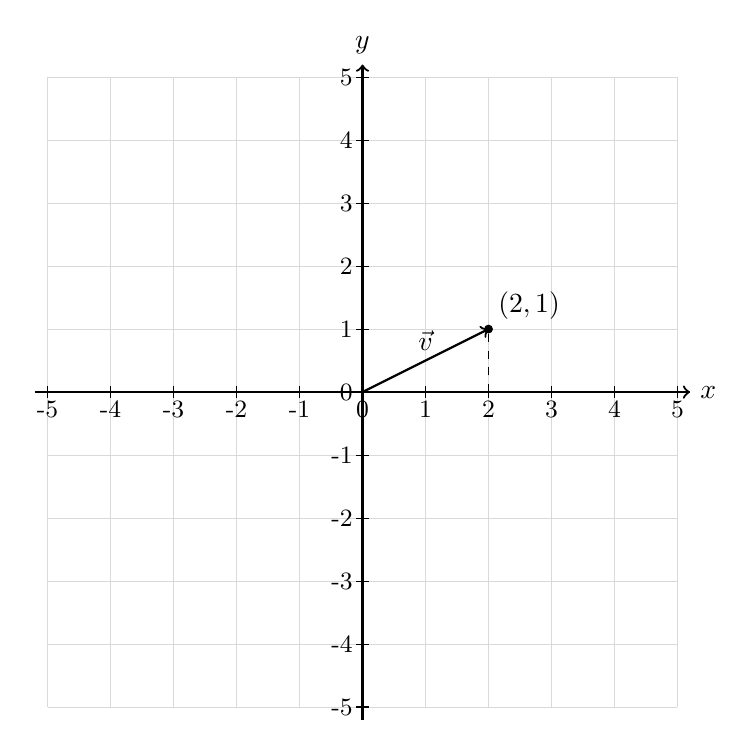
\begin{tikzpicture}[scale=0.8]

        % Grid
        \draw[step=1cm, gray!30, very thin] (-5,-5) grid (5,5);

        % Axes
        \draw[->, thick] (-5.2,0) -- (5.2,0) node[right] {$x$};
        \draw[->, thick] (0,-5.2) -- (0,5.2) node[above] {$y$};

        % Tick marks and labels on x-axis
        \foreach \x in {-5,-4,...,5} {
            \draw (\x,0.1) -- (\x,-0.1);
            \node[below] at (\x,0) {\small \x};
        }

        % Tick marks and labels on y-axis
        \foreach \y in {-5,-4,...,5} {
            \draw (0.1,\y) -- (-0.1,\y);
            \node[left] at (0,\y) {\small \y};
        }

        % Vector
        \draw[->, thick] (0,0) -- (2,1) node[midway, above] {$\vec{v}$};

        % Dashed triangle
        \draw[dashed] (0,0) -- (2,0);
        \draw[dashed] (2,0) -- (2,1);

        % Point
        \fill (2,1) circle (2pt);
        \node[above right] at (2,1) {$(2,1)$};

    \end{tikzpicture}
\end{figure}

Bemærk hvordan der dannes en vektor fra origo ud til punktet (2,1), denne vektor er givet ved:
\begin{equation*}
    \vec{v} = 
    \begin{bmatrix}
        2 \\ 1
    \end{bmatrix}
\end{equation*}

---

\subsection{Længden af en vektor (Pythagoras)}
Hvis vi har en vektor:
\[
\vec{a} =
\begin{bmatrix}
x \\
y
\end{bmatrix}
\]

så svarer længden til hypotenusen i en retvinklet trekant.

\[
|\vec{a}| = \sqrt{x^2 + y^2}
\]

\textbf{Idé:}  
Vi går $x$ til siden og $y$ op → det danner en trekant → Pythagoras.
Dette kommer meget fint ud af vektoren ud til et punkt, længden af den vektor vil altid være hypotenusen af en trekant dannet af x, y værdierne for punktet, deraf kan vektorens længde altid findes ved brug af pythagoras.


---

\subsection{Afstand fra origo til et punkt}
Afstanden fra $(0,0)$ til et punkt $(x,y)$ er derfor:
\[
\sqrt{x^2 + y^2}
\]

Det er altså bare længden af vektoren.

---

\subsection{Afstand mellem to punkter}
Lad os have to punkter:
\[
A = (x_1, y_1), \quad B = (x_2, y_2)
\]

\textbf{Idé:}
1. Lav vektorer fra origo:
\[
\vec{a} =
\begin{bmatrix}
x_1 \\
y_1
\end{bmatrix}
\quad
\vec{b} =
\begin{bmatrix}
x_2 \\
y_2
\end{bmatrix}
\]

2. Træk dem fra hinanden:
\[
\vec{AB} = \vec{b} - \vec{a} =
\begin{bmatrix}
x_2 - x_1 \\
y_2 - y_1
\end{bmatrix}
\]

3. Tag længden:
\[
|AB| = \sqrt{(x_2 - x_1)^2 + (y_2 - y_1)^2}
\]
\textbf{Det er afstandsformlen.}

\begin{figure}[H]
    \centering
    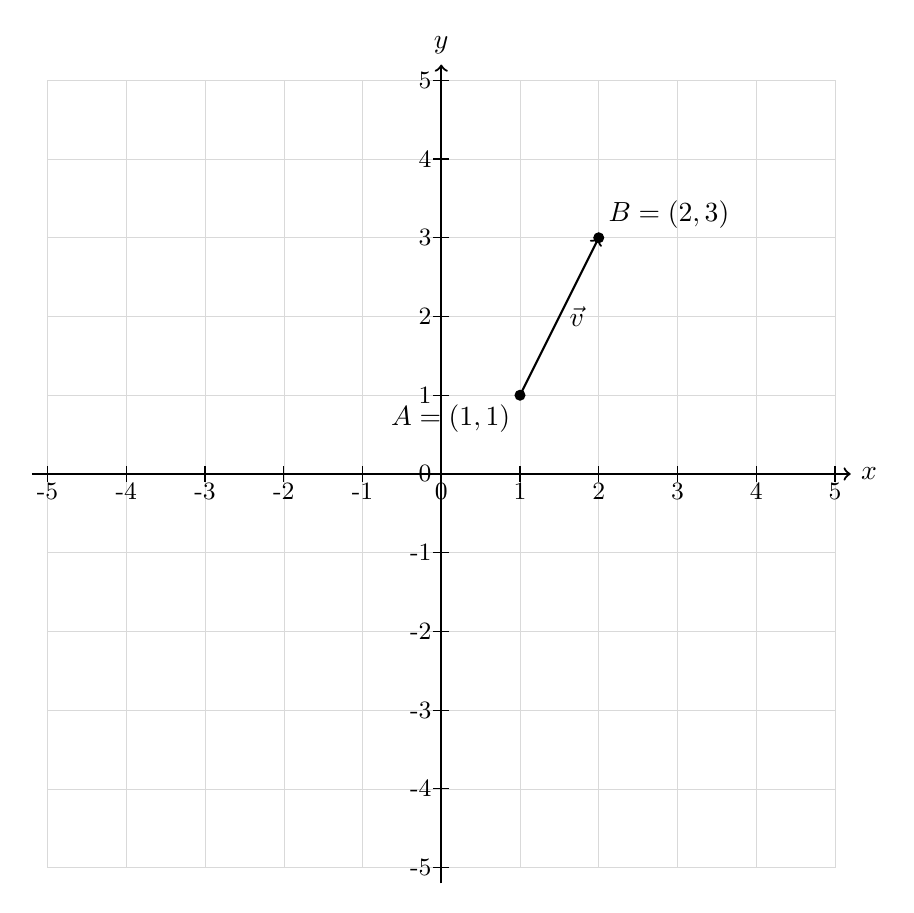
\begin{tikzpicture}[scale=1]

        % Grid
        \draw[step=1cm, gray!30, very thin] (-5,-5) grid (5,5);

        % Axes
        \draw[->, thick] (-5.2,0) -- (5.2,0) node[right] {$x$};
        \draw[->, thick] (0,-5.2) -- (0,5.2) node[above] {$y$};

        % Tick marks and labels on x-axis
        \foreach \x in {-5,-4,...,5} {
            \draw (\x,0.1) -- (\x,-0.1);
            \node[below] at (\x,0) {\small \x};
        }

        % Tick marks and labels on y-axis
        \foreach \y in {-5,-4,...,5} {
            \draw (0.1,\y) -- (-0.1,\y);
            \node[left] at (0,\y) {\small \y};
        }

        % Punkter
        \fill (1,1) circle (2pt);
        \node[below left] at (1,1) {$A=(1,1)$};

        \fill (2,3) circle (2pt);
        \node[above right] at (2,3) {$B=(2,3)$};

        % Vektor
        \draw[->, thick] (1,1) -- (2,3) node[midway, right] {$\vec{v}$};

    \end{tikzpicture}
\end{figure}

Det kan vises lidt mere intuitivt med en figur. Figuren ovenfor viser en vektor fra punktet
$A=(1,1)$ til punktet $B=(2,3)$.

Selve vektoren findes som \textbf{slutpunkt minus startpunkt}, altså:
\begin{equation*}
    \vec{v}
    =
    \begin{bmatrix}
        v_x \\ v_y
    \end{bmatrix}
    =
    \begin{bmatrix}
        B_x-A_x \\
        B_y-A_y
    \end{bmatrix}
    =
    \begin{bmatrix}
        2-1 \\
        3-1
    \end{bmatrix}
    =
    \begin{bmatrix}
        1 \\
        2
    \end{bmatrix}
\end{equation*}

Vi kan altså beskrive en vektor som differensen mellem to punkter. Man kan se det som, at vektoren flyttes, så den starter i origo, uden at den ændrer længde eller retning:

\begin{figure}[H]
    \centering
    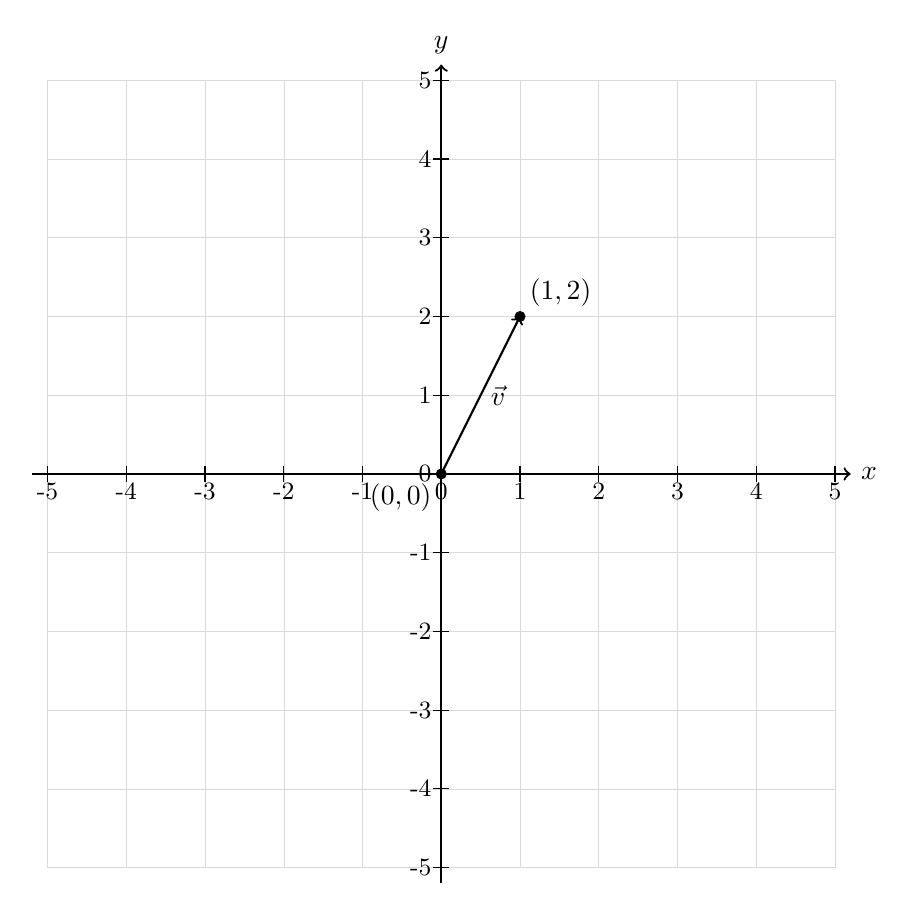
\begin{tikzpicture}[scale=1]

        % Grid
        \draw[step=1cm, gray!30, very thin] (-5,-5) grid (5,5);

        % Axes
        \draw[->, thick] (-5.2,0) -- (5.2,0) node[right] {$x$};
        \draw[->, thick] (0,-5.2) -- (0,5.2) node[above] {$y$};

        % Tick marks and labels on x-axis
        \foreach \x in {-5,-4,...,5} {
            \draw (\x,0.1) -- (\x,-0.1);
            \node[below] at (\x,0) {\small \x};
        }

        % Tick marks and labels on y-axis
        \foreach \y in {-5,-4,...,5} {
            \draw (0.1,\y) -- (-0.1,\y);
            \node[left] at (0,\y) {\small \y};
        }

        % Punkter
        \fill (0,0) circle (2pt);
        \node[below left] at (0,0) {$(0,0)$};

        \fill (1,2) circle (2pt);
        \node[above right] at (1,2) {$(1,2)$};

        % Vektor
        \draw[->, thick] (0,0) -- (1,2) node[midway, right] {$\vec{v}$};

    \end{tikzpicture}
\end{figure}

Når vektoren starter i origo, kan vi bruge Pythagoras som normalt:
\[
|\vec{v}| = \sqrt{1^2+2^2} = \sqrt{5} \approx 2.236
\]

Hele denne proces med at flytte vektoren til origo kan koges ned til én formel. Afstanden mellem to punkter kan derfor skrives som:
\[
|AB| = \sqrt{(B_x-A_x)^2 + (B_y-A_y)^2}
\]

I mange matematikbøger skrives punkterne i stedet som
\[
A=(x_1,y_1), \qquad B=(x_2,y_2)
\]
og så bliver afstandsformlen:
\[
|AB| = \sqrt{(x_2-x_1)^2 + (y_2-y_1)^2}
\]

De to notationer betyder det samme. Notationen med $A_x, A_y, B_x, B_y$ kan dog være nemmere at læse, fordi man tydeligt kan se, hvilken koordinat der hører til hvilket punkt.

---

\subsection{Eksempel}
\[
A = (2,2), \quad B = (4,3)
\]

\[
|AB| = \sqrt{(4-2)^2 + (3-2)^2}
= \sqrt{4 + 1}
= \sqrt{5} \approx 2.24
\]

---

\subsection{Afstand fra punkt til linje}
Hvis vi har en linje:
\[
y = ax + b
\]

og et punkt:
\[
P = (x_0, y_0)
\]

så er afstanden:
\[
\text{dist}(P,l) = \frac{|ax_0 + b - y_0|}{\sqrt{a^2 + 1}}
\]

\textbf{Idé:}
Vi måler den korteste afstand → altså vinkelret ned på linjen.

---

\subsection{Orthogonale linjer (vinkelrette)}
To linjer er orthogonale (vinkelrette), hvis deres hældninger opfylder:
\[
a_1 \cdot a_2 = -1
\]

\textbf{Husk:}
Hvis en linje har hældning $a$, så har den vinkelrette linje hældning:
\[
-\frac{1}{a}
\]

---

\subsection{Eksempel}
Linje:
\[
l: y = 3x - 2
\]

Hældning:
\[
a_l = 3
\]

Vinkelret linje:
\[
a_k = -\frac{1}{3}
\]

Så:
\[
k: y = -\frac{1}{3}x + b
\]

---

\subsection{Opsummering (det vigtigste)}
\begin{itemize}
    \item Vektor = bevægelse fra origo
    \item Længde = Pythagoras
    \item Afstand = længden af forskellen mellem to vektorer
    \item Orthogonale linjer: $a_1 \cdot a_2 = -1$
\end{itemize}